%!TEX root=../document.tex

\section{Einführung}
Diese Uebung soll helfen die Funktionsweise eines Central Authentication Service (CAS). Dabei sollen erste Erfahrung mit den Technologien Single Sign On (SSO) und Ticket Granting Ticket Service (TGT) gemacht werden.

\subsection{Ziele}
Das Ziel dieser Uebung ist die Installation eines CAS-Servers und das Testen einer Anbindung mittels einem CAS-Clients. Die CAS Implementierung basiert auf einem CAS Protokoll, das mit Hilfe von 3 Teilen umgesetzt wird: der CAS-Client (meist ein Webbrowser) stellt eine Anfrage an ein Webapplikation stellt. Die Nutzung der Webapplikation erfordert einen Authentifikation, aus diesem Grund wird der Client an den CAS-Server weitergleitet. Wenn dieser Schritt erfolgreich war, dann wird vom CAS-Server ein Service-Ticket an den Client ausgestellt. Der Client wiederrum leitet das Ticket an die Webapplikation weiter, wo eine sichere Verbindung zwischen Webapplikation und CAS-Server aufgebaut wird, um das Ticket zu prüfen. Wenn diese Validierung erfolgreich war, kann das Resultat der Webapplikation an den Client zurückgegeben werden.

Die CAS-Architektur sieht folgendermassen aus:

\begin{minipage}{\linewidth}
	\centering
	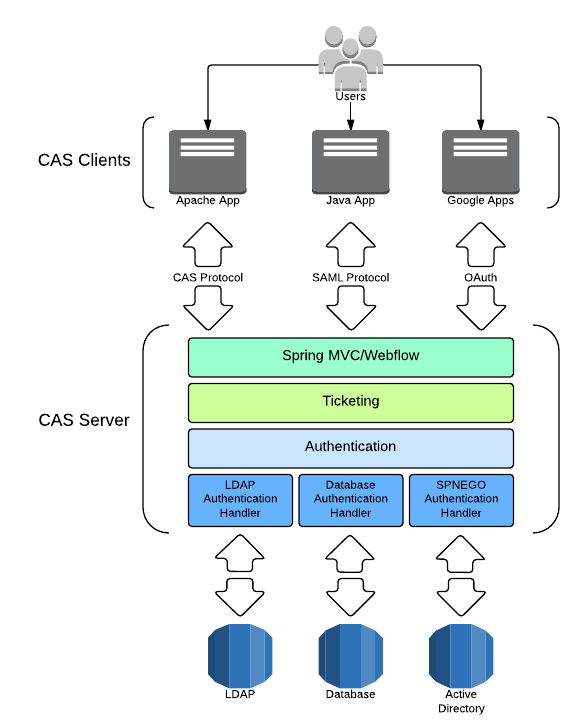
\includegraphics[width=0.59\linewidth]{images/cas_architecture}
	\figcaption{CAS Architektur}
\end{minipage}



\subsection{Voraussetzungen}
\begin{itemize}
	\item Grundlagen zu Central Authentication Service, Single Sign On- und Ticket Granting Ticket Service
	\item Java Programmierkenntnisse
	\item Installation Java JDK 1.8, Apache Tomcat
	\item Installation und Verwendung von Repository Management git
	\item Verwendung von Build Tools maven oder gradle
\end{itemize}


\subsection{Aufgabenstellung}
Installieren Sie eine CAS-Server und probieren Sie damit eine Webapplikation Ihrer Wahl einzubinden.
\begin{itemize}
	\item Download: Apereo CAS 5.0.9
	\item Installation einer Demo Anwendung
	\item Entwicklung einer eigenen Webapplikation, die in der CAS Infrastruktur eingebunden wird
	\item Entwerfen Sie ein Konzept zum Testen der SSO- und TGT-Funktionalität
\end{itemize}
\clearpage
